%-------------------------------------------------------
% SLEPc Users Manual
%-------------------------------------------------------
\chapter{\label{cap:eps}EPS: Eigenvalue Problem Solver}
%-------------------------------------------------------

\noindent The Eigenvalue Problem Solver (\ident{EPS}) is the main object provided by \slepc. It is used to specify a linear eigenvalue problem, either in standard or generalized form, and provides uniform and efficient access to all of the linear eigensolvers included in the package. Conceptually, the level of abstraction occupied by \ident{EPS} is similar to other solvers in \petsc\ such as \ident{KSP} for solving linear systems of equations.

\section{\label{sec:eig}Eigenvalue Problems}

	In this section, we briefly present some basic concepts about eigenvalue problems as well as general techniques used to solve them. The description is not intended to be exhaustive. The objective is simply to define terms that will be referred to throughout the rest of the manual. Readers who are familiar with the terminology and the solution approach can skip this section. For a more comprehensive description, we refer the reader to monographs such as \citep{Stewart:2001:MAV}, \citep{Bai:2000:TSA}, \citep{Saad:1992:NML} or \citep{Parlett:1980:SEP}. A historical perspective of the topic can be found in \citep{Golub:2000:EC2}. See also the \slepc \hyperlink{str}{technical reports}.

In the standard formulation, the linear eigenvalue problem consists in the determination of $\lambda\in\mathbb{C}$ for which the equation
\begin{equation}
Ax=\lambda x\label{eq:eigstd}
\end{equation}
has nontrivial solution, where $A\in\mathbb{C}^{n\times n}$ and $x\in\mathbb{C}^n$. The scalar $\lambda$ and the vector $x$ are called eigenvalue and (right) eigenvector, respectively. Note that they can be complex even when the matrix is real. If $\lambda$ is an eigenvalue of $A$ then $\bar{\lambda}$ is an eigenvalue of its conjugate transpose, $A^*$, or equivalently
\begin{equation}
y^*\!A=\lambda\, y^*,\label{eq:eigstdleft}
\end{equation}
where $y$ is called the left eigenvector.

	In many applications, the problem is formulated as 
\begin{equation}
Ax=\lambda Bx,\label{eq:eiggen}
\end{equation}
where $B\in\mathbb{C}^{n\times n}$, which is known as the generalized eigenvalue problem. Usually, this problem is solved by reformulating it in standard form, for example $B^{-1}Ax=\lambda x$ if $B$ is non-singular.

	\slepc focuses on the solution of problems in which the matrices are large and sparse. Hence, only methods that preserve sparsity are considered.
	These methods obtain the solution from the information generated by the application of the operator to various vectors (the operator is a simple function of matrices $A$ and $B$), that is, matrices are only used in matrix-vector products. This not only maintains sparsity but allows the solution of problems in which matrices are not available explicitly.

In practical analyses, from the $n$ possible solutions, typically only a few eigenpairs $(\lambda,x)$ are considered relevant, either in the extremities of the spectrum, in an interval, or in a region of the complex plane.
Depending on the application, either eigenvalues or eigenvectors or both are required. In some cases, left eigenvectors are also of interest.

\paragraph{Projection Methods.}

	Most eigensolvers provided by \slepc perform a Rayleigh-Ritz projection for extracting the spectral approximations, that is, they project the problem onto a low-dimensional subspace that is built appropriately. Suppose that an orthogonal basis of this subspace is given by $V_j=[v_1,v_2,\ldots,v_j]$. If the solutions of the projected (reduced) problem $B_js=\theta s$ (i.e., $V_j^TAV_j=B_j$) are assumed to be $(\theta_i,s_i)$, $i=1,2,\ldots,j$, then the approximate eigenpairs $(\tilde{\lambda}_i,\tilde{x}_i)$ of the original problem (Ritz value and Ritz vector) are obtained as
\begin{eqnarray}
\tilde{\lambda}_i=\theta_i,\\
\tilde{x}_i=V_js_i.
\end{eqnarray}
Starting from this general idea, eigensolvers differ from each other in which subspace is used, how it is built and other technicalities aimed at improving convergence, reducing storage requirements, etc.

	The subspace
\begin{equation}
\mathcal{K}_m(A,v)\equiv\mathrm{span}\left\{v,Av,A^2v,\ldots,A^{m-1}v\right\},\label{eq:krylov}
\end{equation}
is called the $m$-th Krylov subspace corresponding to $A$ and $v$. Methods that use subspaces of this kind to carry out the projection are called Krylov methods. One example of such methods is the Arnoldi algorithm: starting with $v_1$, $\|v_1\|_2=1$, the Arnoldi basis generation process can be expressed by the recurrence
\begin{equation}
v_{j+1}h_{j+1,j}=w_j=Av_j-\sum_{i=1}^jh_{i,j}v_i,
\end{equation}
where $h_{i,j}$ are the scalar coefficients obtained in the Gram-Schmidt orthogonalization of $Av_j$ with respect to $v_i$, $i=1,2,\ldots,j$, and $h_{j+1,j}=\|w_j\|_2$. Then, the columns of $V_j$ span the Krylov subspace $\mathcal{K}_j(A,v_1)$ and $Ax=\lambda x$ is projected into $H_js=\theta s$, where $H_j$ is an upper Hessenberg matrix with elements $h_{i,j}$, which are 0 for $i\geq j+2$. The related Lanczos algorithms obtain a projected matrix that is tridiagonal.

	A generalization to the above methods are the block Krylov strategies, in which the starting vector $v_1$ is replaced by a full rank $n\times p$ matrix $V_1$, which allows for better convergence properties when there are multiple eigenvalues and can provide better data management on some computer architectures. Block tridiagonal and block Hessenberg matrices are then obtained as projections.

	It is generally assumed (and observed) that the Lanczos and Arnoldi algorithms find solutions at the extremities of the spectrum. Their convergence pattern, however, is strongly related to the eigenvalue distribution. Slow convergence may be experienced in the presence of tightly clustered eigenvalues. The maximum allowable $j$ may be reached without having achieved convergence for all desired solutions. Then, restarting is usually a useful technique and different strategies exist for that purpose. However, convergence can still be very slow and acceleration strategies must be applied. Usually, these techniques consist in computing eigenpairs of a transformed operator and then recovering the solution of the original problem. The aim of these transformations is twofold. On one hand, they make it possible to obtain eigenvalues other than those lying in the boundary of the spectrum. On the other hand, the separation of the eigenvalues of interest is improved in the transformed spectrum thus leading to faster convergence. The most commonly used spectral transformation is called shift-and-invert, which works with operator $(A-\sigma I)^{-1}$. It allows the computation of eigenvalues closest to $\sigma$ with very good separation properties. When using this approach, a linear system of equations, $(A-\sigma I)y=x$, must be solved in each iteration of the eigenvalue process.

\paragraph{Preconditioned Eigensolvers.}
	In many applications, Krylov eigensolvers perform very well because Krylov subspaces are optimal in a certain theoretical sense. However, these methods may not be appropriate in some situations such as the computation of interior eigenvalues. The spectral transformation mentioned above may not be a viable solution or it may be too costly. For these reasons, other types of eigensolvers such as Davidson and Jacobi-Davidson rely on a different way of expanding the subspace. Instead of satisfying the Krylov relation, these methods compute the new basis vector by the so-called correction equation. The resulting subspace may be richer in the direction of the desired eigenvectors. These solvers may be competitive especially for computing interior eigenvalues. From a practical point of view, the correction equation may be seen as a cheap replacement for the shift-and-invert system of equations, $(A-\sigma I)y=x$. By cheap we mean that it may be solved inaccurately without compromising robustness, via a preconditioned iterative linear solver. For this reason, these are known as \emph{preconditioned} eigensolvers.

\paragraph{Related Problems.}

	In many applications such as the analysis of damped vibrating systems the problem to be solved is a \emph{quadratic eigenvalue problem} (QEP), or more generally a \emph{nonlinear eigenvalue problem} (NEP). For these, the reader is referred to chapters \ref{cap:pep} and \ref{cap:nep}. Another linear algebra problem that is very closely related to the eigenvalue problem is the {\em singular value decomposition\/} (SVD), see chapter \ref{cap:svd}. 

%---------------------------------------------------
\section{Basic Usage}

	The \ident{EPS} module in \slepc is used in a similar way as \petsc modules such as \ident{KSP}. All the information related to an eigenvalue problem is handled via a context variable. The usual object management functions are available (\ident{EPSCreate}, \ident{EPSDestroy}, \ident{EPSView}, \ident{EPSSetFromOptions}). In addition, the \ident{EPS} object provides functions for setting several parameters such as the number of eigenvalues to compute, the dimension of the subspace, the portion of the spectrum of interest, the requested tolerance or the maximum number of iterations allowed.

	The solution of the problem is obtained in several steps. First of all, the matrices associated with the eigenproblem are specified via \ident{EPSSetOperators} and \ident{EPSSetProblemType} is used to specify the type of problem. Then, a call to \ident{EPSSolve} is done that invokes the subroutine for the selected eigensolver. \ident{EPSGetConverged} can be used afterwards to determine how many of the requested eigenpairs have converged to working accuracy. \ident{EPSGetEigenpair} is finally used to retrieve the eigenvalues and eigenvectors.

	In order to illustrate the basic functionality of the \ident{EPS} package, a simple example is shown in Figure \ref{fig:ex-eps}. The example code implements the solution of a simple standard eigenvalue problem. Code for setting up the matrix $A$ is not shown and error-checking code is omitted.

\begin{figure}
\begin{Verbatim}[fontsize=\small,numbers=left,numbersep=6pt,xleftmargin=15mm]
EPS         eps;       /*  eigensolver context  */
Mat         A;         /*  matrix of Ax=kx      */
Vec         xr, xi;    /*  eigenvector, x       */
PetscScalar kr, ki;    /*  eigenvalue, k        */
PetscInt    j, nconv;
PetscReal   error;

EPSCreate( PETSC_COMM_WORLD, &eps );
EPSSetOperators( eps, A, NULL );
EPSSetProblemType( eps, EPS_NHEP );
EPSSetFromOptions( eps );
EPSSolve( eps );
EPSGetConverged( eps, &nconv );
for (j=0; j<nconv; j++) {
  EPSGetEigenpair( eps, j, &kr, &ki, xr, xi );
  EPSComputeRelativeError( eps, j, &error );
}
EPSDestroy( &eps );
\end{Verbatim}
\caption{\label{fig:ex-eps}Example code for basic solution with \ident{EPS}.}
\end{figure}

	All the operations of the program are done over a single \ident{EPS} object. This solver context is created in line 8 with the command 
	\findex{EPSCreate}
	\begin{Verbatim}[fontsize=\small]
	EPSCreate(MPI_Comm comm,EPS *eps);
	\end{Verbatim}
	Here \texttt{comm} is the MPI communicator, and \texttt{eps} is the newly formed solver context. The communicator indicates which processes are involved in the \ident{EPS} object. Most of the \ident{EPS} operations are collective, meaning that all the processes collaborate to perform the operation in parallel. 

	Before actually solving an eigenvalue problem with \ident{EPS}, the user must specify the matrices associated with the problem, as in line 9, with the following routine
	\findex{EPSSetOperators}
	\begin{Verbatim}[fontsize=\small]
	EPSSetOperators(EPS eps,Mat A,Mat B);
	\end{Verbatim}
	The example specifies a standard eigenproblem. In the case of a generalized problem, it would be necessary also to provide matrix $B$ as the third argument to the call. The matrices specified in this call can be in any \petsc format. In particular, \ident{EPS} allows the user to solve matrix-free problems by specifying matrices created via \ident{MatCreateShell}. A more detailed discussion of this issue is given in \S\ref{sec:supported}.

	After setting the problem matrices, the problem type is set with \ident{EPSSetProblemType}. This is not strictly necessary since if this step is skipped then the problem type is assumed to be non-symmetric. More details are given in \S\ref{sec:defprob}.
	At this point, the value of the different options could optionally be set by means of a function call such as \ident{EPSSetTolerances} (explained later in this chapter). After this, a call to \ident{EPSSetFromOptions} should be made as in line 11, 
	\findex{EPSSetFromOptions}
	\begin{Verbatim}[fontsize=\small]
	EPSSetFromOptions(EPS eps);
	\end{Verbatim}
	The effect of this call is that options specified at runtime in the command line are passed to the \ident{EPS} object appropriately. In this way, the user can easily experiment with different combinations of options without having to recompile. All the available options as well as the associated function calls are described later in this chapter.

	Line 12 launches the solution algorithm, simply with the command
	\findex{EPSSolve}
	\begin{Verbatim}[fontsize=\small]
	EPSSolve(EPS eps);
	\end{Verbatim}
	The subroutine that is actually invoked depends on which solver has been selected by the user. 
        
        After the call to \ident{EPSSolve} has finished, all the data associated with the solution of the eigenproblem is kept internally. This information can be retrieved with different function calls, as in lines 13 to 17. This part is described in detail in \S\ref{sec:retrsol}.

	Once the \ident{EPS} context is no longer needed, it should be destroyed with the command
	\findex{EPSDestroy}
	\begin{Verbatim}[fontsize=\small]
	EPSDestroy(EPS *eps);
	\end{Verbatim}

	The above procedure is sufficient for general use of the \ident{EPS} package. As in the case of the \ident{KSP} solver, the user can optionally explicitly call 
	\findex{EPSSetUp}
	\begin{Verbatim}[fontsize=\small]
	EPSSetUp(EPS eps);
	\end{Verbatim}
before calling \ident{EPSSolve} to perform any setup required for the eigensolver.

	Internally, the \ident{EPS} object works with an \ident{ST} object (spectral transformation, described in chapter \ref{cap:st}). To allow application programmers to set any of the spectral transformation options directly within the code, the following routine is provided to extract the \ident{ST} context,
	\findex{EPSGetST}
	\begin{Verbatim}[fontsize=\small]
	EPSGetST(EPS eps,ST *st);
	\end{Verbatim}
	
	With the command
	\findex{EPSView}
	\begin{Verbatim}[fontsize=\small]
	EPSView(EPS eps,PetscViewer viewer);
	\end{Verbatim}
it is possible to examine the actual values of the different settings of the \ident{EPS} object, including also those related to the associated \ident{ST} object. This is useful for making sure that the solver is using the settings that the user wants.

%---------------------------------------------------
\section{Defining the Problem}
\label{sec:defprob}

	\slepc is able to cope with different kinds of problems. Currently supported problem types are listed in Table \ref{tab:ptype}. An eigenproblem is generalized ($Ax=\lambda Bx$) if the user has specified two matrices (see \ident{EPSSetOperators} above), otherwise it is standard ($Ax=\lambda x$). A standard eigenproblem is Hermitian if matrix $A$ is Hermitian (i.e., $A=A^*$) or, equivalently in the case of real matrices, if matrix $A$ is symmetric (i.e., $A=A^T$). A generalized eigenproblem is Hermitian if matrix $A$ is Hermitian (symmetric) and $B$ is Hermitian (symmetric) and positive (semi-)definite.
If $B$ is not positive (semi-)definite then the problem cannot be considered Hermitian but symmetry can still be exploited to some extent in some solvers (problem type \texttt{EPS\_GHIEP}).
A special case of generalized non-Hermitian problem is when $A$ is non-Hermitian but $B$ is Hermitian and positive (semi-)definite, see \S\ref{sec:symm} and \S\ref{sec:purif} for discussion.

\begin{table}[t]
\centering
{\small \begin{tabular}{lll}
Problem Type              & \ident{EPSProblemType}    & Command line key\\\hline
Hermitian                 & \texttt{EPS\_HEP}         & \texttt{-eps\_hermitian}\\
Non-Hermitian             & \texttt{EPS\_NHEP}        & \texttt{-eps\_non\_hermitian}\\
Generalized Hermitian     & \texttt{EPS\_GHEP}        & \texttt{-eps\_gen\_hermitian}\\
Generalized Hermitian indefinite & \texttt{EPS\_GHIEP} & \texttt{-eps\_gen\_indefinite}\\
Generalized Non-Hermitian & \texttt{EPS\_GNHEP}       & \texttt{-eps\_gen\_non\_hermitian}\\
GNHEP with positive (semi-)definite $B$ & \texttt{EPS\_PGNHEP} & \texttt{-eps\_pos\_gen\_non\_hermitian}\\\hline
\end{tabular} }
\caption{\label{tab:ptype}Problem types considered in \ident{EPS}.}
\end{table}

The problem type can be specified at run time with the corresponding command line key or, more usually, within the program with the function
	\findex{EPSSetProblemType}
	\begin{Verbatim}[fontsize=\small]
	EPSSetProblemType(EPS eps,EPSProblemType type);
	\end{Verbatim}

By default, \slepc assumes that the problem is non-Hermitian. Some eigensolvers are able to exploit symmetry, that is, they compute a solution for Hermitian problems with less storage and/or computational cost than other methods that ignore this property. Also, symmetric solvers may be more accurate. On the other hand, some eigensolvers in \slepc only have a symmetric version and will abort if the problem is non-Hermitian. 
In the case of generalized eigenproblems some considerations apply regarding symmetry, especially in the case of singular $B$. This topic is tackled in \S\ref{sec:symm} and \S\ref{sec:purif}.
For all these reasons, the user is strongly recommended to always specify the problem type in the source code. 

	The type of the problem can be determined with the functions
	\findex{EPSIsGeneralized} \findex{EPSIsHermitian}
	\begin{Verbatim}[fontsize=\small]
	EPSIsGeneralized(EPS eps,PetscBool *gen);
	EPSIsHermitian(EPS eps,PetscBool *her);
	EPSIsPositive(EPS eps,PetscBool *pos);
	\end{Verbatim}

	The user can specify how many eigenvalues (and eigenvectors) to compute. The default is to compute only one. The function
	\findex{EPSSetDimensions}
	\begin{Verbatim}[fontsize=\small]
	EPSSetDimensions(EPS eps,PetscInt nev,PetscInt ncv,PetscInt mpd);
	\end{Verbatim}
allows the specification of the number of eigenvalues to compute, \texttt{nev}. The second argument can be set to prescribe the number of column vectors to be used by the solution algorithm, \texttt{ncv}, that is, the largest dimension of the working subspace. The third argument has to do with a more advanced usage, as explained in \S\ref{sec:large-nev}. These parameters can also be set at run time with the options \Verb!-eps_nev!, \Verb!-eps_ncv! and \Verb!-eps_mpd!. For example, the command line
\begin{Verbatim}[fontsize=\small]
	$ ./program -eps_nev 10 -eps_ncv 24
\end{Verbatim}
requests 10 eigenvalues and instructs to use 24 column vectors. Note that \texttt{ncv} must be at least equal to \texttt{nev}, although in general it is recommended (depending on the method) to work with a larger subspace, for instance $\mathtt{ncv}\geq2\cdot\mathtt{nev}$ or even more. The case that the user requests a relatively large number of eigenpairs is discussed in \S\ref{sec:large-nev}.

\paragraph{Eigenvalues of Interest.}

	For the selection of the portion of the spectrum of interest, there are several alternatives. In real symmetric problems, one may want to compute the largest or smallest eigenvalues in magnitude, or the leftmost or rightmost ones, or even all eigenvalues in a given interval. In other problems, in which the eigenvalues can be complex, then one can select eigenvalues depending on the magnitude, or the real part or even the imaginary part. Sometimes the eigenvalues of interest are those closest to a given target value, $\tau$, measuring the distance either in the ordinary way or along the real (or imaginary) axis. Table \ref{tab:portion} summarizes all the possibilities available for the function
	\findex{EPSSetWhichEigenpairs}
	\begin{Verbatim}[fontsize=\small]
	EPSSetWhichEigenpairs(EPS eps,EPSWhich which);
	\end{Verbatim}
which can also be specified at the command line. This criterion is used both for configuring how the eigensolver seeks eigenvalues (note that not all these possibilities are available for all the solvers) and also for sorting the computed values. The default is to compute the largest magnitude eigenvalues, except for those solvers in which this option is not available. There is another exception related to the use of some spectral transformations, see chapter \ref{cap:st}.

	For the sorting criteria relative to a target value, the following function must be called in order to specify such value $\tau$:
	\findex{EPSSetTarget}
	\begin{Verbatim}[fontsize=\small]
	EPSSetTarget(EPS eps,PetscScalar target);
	\end{Verbatim}
or, alternatively, with the command-line key \Verb!-eps_target!. Note that, since the target is defined as a \texttt{PetscScalar}, complex values of $\tau$ are allowed only in the case of complex scalar builds of the SLEPc library.

The use of a target value makes sense if the eigenvalues of interest are located in the interior of the spectrum. Since these eigenvalues are usually more difficult to compute, the eigensolver by itself may not be able to obtain them, and additional tools are normally required. 
There are two possibilities for this:
\begin{itemize}
\item To use harmonic extraction (see \S\ref{sec:harmonic}), a variant of some solvers that allows a better approximation of interior eigenvalues without changing the way the subspace is built.
\item To use a spectral transformation such as shift-and-invert (see chapter \ref{cap:st}), where the subspace is built from a transformed problem (usually much more costly).
\end{itemize}

The special case of computing all eigenvalues in an interval is discussed in \S\ref{sec:slice}, since it is related also to spectral transformations. In this case, instead of a target value the user has to specify the computational interval with
	\findex{EPSSetInterval}
	\begin{Verbatim}[fontsize=\small]
	EPSSetInterval(EPS eps,PetscScalar a,PetscScalar b);
	\end{Verbatim}
which is equivalent to \Verb!-eps_interval <a,b>!.

Finally, we mention the possibility of defining an arbitrary sorting criterion by means of \texttt{EPS\_WHICH\_USER} in combination with \ident{EPSSetEigenvalueComparison}.

\begin{table}
\centering
{\small \begin{tabular}{lll}
\texttt{EPSWhich}                  & Command line key                   & Sorting criterion \\\hline
\texttt{EPS\_LARGEST\_MAGNITUDE}   & \texttt{-eps\_largest\_magnitude}  & Largest $|\lambda|$ \\
\texttt{EPS\_SMALLEST\_MAGNITUDE}  & \texttt{-eps\_smallest\_magnitude} & Smallest $|\lambda|$ \\
\texttt{EPS\_LARGEST\_REAL}        & \texttt{-eps\_largest\_real}       & Largest $\mathrm{Re}(\lambda)$ \\
\texttt{EPS\_SMALLEST\_REAL}       & \texttt{-eps\_smallest\_real}      & Smallest $\mathrm{Re}(\lambda)$ \\
\texttt{EPS\_LARGEST\_IMAGINARY}   & \texttt{-eps\_largest\_imaginary}  & Largest $\mathrm{Im}(\lambda)$\footnotemark \\
\texttt{EPS\_SMALLEST\_IMAGINARY}  & \texttt{-eps\_smallest\_imaginary} & Smallest $\mathrm{Im}(\lambda)$\addtocounter{footnote}{-1}\footnotemark \\
\hline
\texttt{EPS\_TARGET\_MAGNITUDE}    & \texttt{-eps\_target\_magnitude}   & Smallest $|\lambda-\tau|$ \\
\texttt{EPS\_TARGET\_REAL}         & \texttt{-eps\_target\_real}        & Smallest $|\mathrm{Re}(\lambda-\tau)|$ \\
\texttt{EPS\_TARGET\_IMAGINARY}    & \texttt{-eps\_target\_imaginary}   & Smallest $|\mathrm{Im}(\lambda-\tau)|$ \\
\texttt{EPS\_ALL}                  & \texttt{-eps\_all}                 & All $\lambda\in[a,b]$ \\
\hline
\texttt{EPS\_WHICH\_USER}          &                                    & \emph{user-defined} \\\hline
\end{tabular} }
\caption{\label{tab:portion}Available possibilities for selection of the eigenvalues of interest.}
\end{table}

\footnotetext{If \slepc is compiled for real scalars, then the absolute value of the imaginary part, $|\mathrm{Im}(\lambda)|$, is used for eigenvalue selection and sorting.}

The selection criteria discussed above are based solely on the eigenvalue. In some special situations, it is necessary to establish a user-defined criterion that also makes use of the eigenvector when deciding which are the most wanted eigenpairs. For these cases, use \ident{EPSSetArbitrarySelection}.

%---------------------------------------------------
\section{Selecting the Eigensolver}

	The available methods for solving the eigenvalue problems are the following:
\begin{itemize}
\setlength{\itemsep}{0pt}
\item Power Iteration with deflation. When combined with shift-and-invert (see chapter \ref{cap:st}), it is equivalent to the Inverse Iteration. Also, this solver embeds the Rayleigh Quotient Iteration (RQI) by allowing variable shifts.
\item Subspace Iteration with Rayleigh-Ritz projection and locking.
\item Arnoldi method with explicit restart and deflation.
\item Lanczos with explicit restart and deflation, using different reorthogonalization strategies.
\item Krylov-Schur, a variation of Arnoldi with a very effective restarting technique. In the case of symmetric problems, this is equivalent to the thick-restart Lanczos method.
\item Generalized Davidson, a simple iteration based on the subspace expansion by the preconditioned residual.
\item Jacobi-Davidson, a preconditioned eigensolver with an effective correction equation.
\item RQCG, a basic conjugate gradient iteration for the minimization of the Rayleigh quotient.
\item CISS, a contour-integral solver that allows computing all eigenvalues in a given region.
\end{itemize}

\begin{table}
\centering
{\small \begin{tabular}{lllc}
                           &                      & {\footnotesize Options} & \\
Method                     & \ident{EPSType}      & {\footnotesize Database Name} & Default\\\hline
Power / Inverse / RQI      & \texttt{EPSPOWER}    & \texttt{power} \\
Subspace Iteration         & \texttt{EPSSUBSPACE} & \texttt{subspace} \\
Arnoldi                    & \texttt{EPSARNOLDI}  & \texttt{arnoldi} \\
Lanczos                    & \texttt{EPSLANCZOS}  & \texttt{lanczos} \\
Krylov-Schur               & \texttt{EPSKRYLOVSCHUR} & \texttt{krylovschur} & $\star$ \\
Generalized Davidson       & \texttt{EPSGD}       & \texttt{gd} \\
Jacobi-Davidson            & \texttt{EPSJD}       & \texttt{jd} \\
Rayleigh quotient CG       & \texttt{EPSRQCG}     & \texttt{rqcg} \\
Contour integral SS        & \texttt{EPSCISS}     & \texttt{ciss} \\
\hline
\lapack solver             & \texttt{EPSLAPACK}   & \texttt{lapack} \\
Wrapper to \arpack         & \texttt{EPSARPACK}   & \texttt{arpack} \\
Wrapper to \primme         & \texttt{EPSPRIMME}   & \texttt{primme} \\
Wrapper to \blzpack        & \texttt{EPSBLZPACK}  & \texttt{blzpack} \\
Wrapper to \trlan          & \texttt{EPSTRLAN}    & \texttt{trlan} \\
Wrapper to \blopex         & \texttt{EPSBLOPEX}   & \texttt{blopex} \\
Wrapper to \feast          & \texttt{EPSFEAST}    & \texttt{feast} \\\hline
\end{tabular} }
\caption{\label{tab:solvers}Eigenvalue solvers available in the \ident{EPS} module.}
\end{table}

The default solver is Krylov-Schur. A detailed description of the implemented algorithms is provided in the \hyperlink{str}{\slepc Technical Reports}. In addition to these methods, \slepc also provides wrappers to external packages such as \arpack, \blzpack, or \trlan. A complete list of these interfaces can be found in \S\ref{sec:wrap}.

As an alternative, \slepc provides an interface to some \lapack routines. These routines operate in dense mode with only one processor and therefore are suitable only for moderate size problems. This solver should be used only for debugging purposes.

The solution method can be specified procedurally or via the command line. The application programmer can set it by means of the command
	\findex{EPSSetType}
	\begin{Verbatim}[fontsize=\small]
	EPSSetType(EPS eps,EPSType method);
	\end{Verbatim}
while the user writes the options database command \Verb!-eps_type! followed by the name of the method (see Table \ref{tab:solvers}).

	Not all the methods can be used for all problem types. Table \ref{tab:support} summarizes the scope of each eigensolver by listing which portion of the spectrum can be selected (as defined in Table \ref{tab:portion}), which problem types are supported (as defined in Table \ref{tab:ptype}) and whether they are available or not in the complex version of \slepc. Also, the default value of some parameters differ from one solver to the other, as shown in Table \ref{tab:defaults}. This table also illustrates the different storage requirements. All solvers need memory at least for storing $ncv$ vectors, but in addition some extra work storage such as auxiliary vectors is necessary. The last columns of Table \ref{tab:defaults} indicates the number of auxiliary vectors required in each case.

\begin{table}
\centering
\begin{tabular}{ccccc} \hline
Method   &  Portion of spectrum & Problem type & Real/Complex \\ \hline
\texttt{power}       & Largest $|\lambda|$ & any & both \\ 
\texttt{subspace}    & Largest $|\lambda|$ & any & both \\ 
\texttt{arnoldi}     & any\footnotemark    & any & both\addtocounter{footnote}{-1} \\ 
\texttt{lanczos}     & any\footnotemark    & \Verb!EPS_HEP!, \Verb!EPS_GHEP! & both\addtocounter{footnote}{-1} \\ 
\texttt{krylovschur} & any                 & any & both \\ 
\texttt{gd}          & any\footnotemark    & any & both\addtocounter{footnote}{-1} \\ 
\texttt{jd}          & any\footnotemark    & any & both\addtocounter{footnote}{-1} \\ 
\texttt{rqcg}        & Smallest $\mathrm{Re}(\lambda)$ & \Verb!EPS_HEP!, \Verb!EPS_GHEP! & both \\ 
\texttt{ciss}        & All $\lambda$ in region & any & complex \\ 
\hline
\texttt{lapack}      & any                 & any & both \\ 
\texttt{arpack}      & any\footnotemark    & any & both \\ 
\texttt{primme}      & Largest and smallest $\mathrm{Re}(\lambda)$ & \Verb!EPS_HEP! & both \\ 
\texttt{blzpack}     & Smallest $\mathrm{Re}(\lambda)$ & \Verb!EPS_HEP!, \Verb!EPS_GHEP!  & real \\ 
\texttt{trlan}       & Largest and smallest $\mathrm{Re}(\lambda)$ & \Verb!EPS_HEP! & real \\
\texttt{blopex}      & Smallest $\mathrm{Re}(\lambda)$ & \Verb!EPS_HEP!, \Verb!EPS_GHEP! & both \\
\texttt{feast}       & All $\lambda$ in an interval & \Verb!EPS_HEP!, \Verb!EPS_GHEP! & complex \\ \hline
\end{tabular}
\caption{\label{tab:support}Supported problem types for all eigensolvers available in \slepc.}
\end{table}

\footnotetext{Any of the selection criteria except for \texttt{EPS\_ALL}, which is supported only by Krylov-Schur; see \S\ref{sec:slice}.}

\begin{table}[t!]
\centering
\begin{tabular}{cccc} \hline
Method   & \texttt{ncv} & \texttt{max\_it} & Storage \\ \hline
\texttt{power}    &  $nev$ & $\max(2000,100N)$ & $2$ \\ 
\texttt{subspace} &  $\max(2\cdot nev,nev+15)$ & $\max(100,\lceil 2N/ncv \rceil)$ & $ncv$ \\ 
\texttt{arnoldi}  &  $\max(2\cdot nev,nev+15)$ & $\max(100,\lceil 2N/ncv \rceil)$ & $1$ \\ 
\texttt{lanczos}  &  $\max(2\cdot nev,nev+15)$ & $\max(100,\lceil 2N/ncv \rceil)$ & $1$ \\ 
\texttt{krylovschur} & $\max(2\cdot nev,nev+15)$ & $\max(100,\lceil 2N/ncv \rceil)$ & $1$ \\ 
\texttt{gd}       & $\max(2\cdot nev,nev+15)+1$ & $\max(100,\lceil 2N/ncv \rceil)$ & $4ncv+1$ \\ 
\texttt{jd}       & $\max(2\cdot nev,nev+15)+1$ & $\max(100,\lceil 2N/ncv \rceil)$ & $4ncv+1$ \\ 
\texttt{rqcg} & $\max(2\cdot nev,nev+15)$ & $\max(100,\lceil 2N/ncv \rceil)$ & $4ncv$ \\ 
\hline
\texttt{lapack}   &  $N$ &         -         & $N$  \\ 
\texttt{arpack}   &  $\max(20,2\!\cdot\!nev\!+\!\!1)$ & $\max(300,\lceil 2N/ncv\rceil)$ & $4$ \\ 
\texttt{primme}   &  $\max(20,2\!\cdot\!nev\!+\!\!1)$ & $\max(1000,N)$ & $3$ \\ 
\texttt{blzpack}  &  $\min(nev\!+\!\!10,2\!\cdot\!nev)$ & $\max(1000,N)$ & $>187$ \\ 
\texttt{trlan}    &  $nev$ & $\max(1000,N)$ & $nev+1$ \\
\texttt{blopex}   &  $nev$ & $\max(100,\lceil 2N/ncv \rceil)$ & $nev$ \\ \hline
\end{tabular}
\caption{\label{tab:defaults}Default parameter values for all eigensolvers available in \slepc.}
\end{table}

%---------------------------------------------------
\section{Retrieving the Solution}
\label{sec:retrsol}

Once the call to \ident{EPSSolve} is complete, all the data associated with the solution of the eigenproblem is kept internally in the \ident{EPS} object. This information can be obtained by the calling program by means of a set of functions described in this section.

	As explained below, the number of computed solutions depends on the convergence and, therefore, it may be different from the number of solutions requested by the user. So the first task is to find out how many solutions are available, with
	\findex{EPSGetConverged}
	\begin{Verbatim}[fontsize=\small]
	EPSGetConverged(EPS eps,PetscInt *nconv);
	\end{Verbatim}
Usually, the number of converged solutions, \texttt{nconv}, will be equal to \texttt{nev}, but in general it will be a number ranging from 0 to \texttt{ncv} (here, \texttt{nev} and \texttt{ncv} are the arguments of function \ident{EPSSetDimensions}).

\subsection{The Computed Solution}

	The user may be interested in the eigenvalues, or the eigenvectors, or both. The function
	\findex{EPSGetEigenpair}
	\begin{Verbatim}[fontsize=\small]
	EPSGetEigenpair(EPS eps,PetscInt j,PetscScalar *kr,PetscScalar *ki,
                        Vec xr,Vec xi);
	\end{Verbatim}
	\label{GetEigenpair}
returns the $j$-th computed eigenvalue/eigenvector pair. Typically, this function is called inside a loop for each value of \texttt{j} from 0 to \texttt{nconv}--1. Note that eigenvalues are ordered according to the same criterion specified with function \ident{EPSSetWhichEigenpairs} for selecting the portion of the spectrum of interest.
	The meaning of the last 4 parameters depends on whether \slepc has been compiled for real or complex scalars, as detailed below. The eigenvectors are normalized so that they have a unit 2-norm, except for problem type \ident{EPS\_GHEP} in which case returned eigenvectors have a unit $B$-norm.

\paragraph{Real \slepc.} In this case, all \texttt{Mat} and \texttt{Vec} objects are real. The computed approximate solution returned by the function \ident{EPSGetEigenpair} is stored in the following way: \texttt{kr} and \texttt{ki} contain the real and imaginary parts of the eigenvalue, respectively, and \texttt{xr} and \texttt{xi} contain the associated eigenvector. Two cases can be distinguished:

\begin{itemize}
\item When \texttt{ki} is zero, it means that the $j$-th eigenvalue is a real number. In this case, \texttt{kr} is the eigenvalue and \texttt{xr} is the corresponding eigenvector. The vector \texttt{xi} is set to all zeros.

\item If \texttt{ki} is different from zero, then the $j$-th eigenvalue is a complex number and, therefore, it is part of a complex conjugate pair. Thus, the $j$-th eigenvalue is \texttt{kr}$+\,i\cdot$\texttt{ki}.
With respect to the eigenvector, \texttt{xr} stores the real part of the eigenvector and \texttt{xi} the imaginary part, that is, the $j$-th eigenvector is \texttt{xr}$+\,i\cdot$\texttt{xi}. The $(j+1)$-th eigenvalue (and eigenvector) will be the corresponding complex conjugate and will be returned when function \ident{EPSGetEigenpair} is invoked with index \texttt{j}+1. Note that the sign of the imaginary part is returned correctly in all cases (users need not change signs).
\end{itemize}

\paragraph{Complex \slepc.} In this case, all \texttt{Mat} and \texttt{Vec} objects are complex. The computed solution returned by function \ident{EPSGetEigenpair} is the following: \texttt{kr} contains the (complex) eigenvalue and \texttt{xr} contains the corresponding (complex) eigenvector. In this case, \texttt{ki} and \texttt{xi} are not used (set to all zeros).

\subsection{Reliability of the Computed Solution}
\label{sec:errbnd}

	In this subsection, we discuss how a-posteriori error bounds can be obtained in order to assess the accuracy of the computed solutions. These bounds are based on the so-called residual vector, defined as
\begin{equation}
r=A\tilde{x}-\tilde{\lambda}\tilde{x},
\end{equation}
or $r=A\tilde{x}-\tilde{\lambda}B\tilde{x}$ in the case of a generalized problem, where $\tilde{\lambda}$ and $\tilde{x}$ represent any of the \texttt{nconv} computed eigenpairs delivered by \texttt{EPSGetEigenpair} (note that this function returns a normalized $\tilde{x}$). 

	In the case of Hermitian problems, it is possible to demonstrate the following property (see for example \citep[ch. 3]{Saad:1992:NML}):
\begin{equation}\label{eq:reserr}
|\lambda-\tilde{\lambda}|\leq \|r\|_2,
\end{equation}
where $\lambda$ is an exact eigenvalue. Therefore, the 2-norm of the residual vector can be used as a bound for the absolute error in the eigenvalue.

	In the case of non-Hermitian problems, the situation is worse because no simple relation such as Eq.\ \ref{eq:reserr} is available. This means that in this case the residual norms may still give an indication of the actual error but the user should be aware that they may sometimes be completely wrong, especially in the case of highly non-normal matrices. A better bound would involve also the residual norm of the left eigenvector.

	With respect to eigenvectors, we have a similar scenario in the sense that bounds for the error may be established in the Hermitian case only, for example the following one:
\begin{equation}
\sin \theta(x,\tilde{x})\leq \frac{\|r\|_2}{\delta},
\end{equation}
where $\theta(x,\tilde{x})$ is the angle between the computed and exact eigenvectors, and $\delta$ is the distance from $\tilde{\lambda}$ to the rest of the spectrum. This bound is not provided by \slepc because $\delta$ is not available. The above expression is given here simply to warn the user about the fact that accuracy of eigenvectors may be deficient in the case of clustered eigenvalues.

	In the case of non-Hermitian problems, \slepc provides the alternative of retrieving an orthonormal basis of an invariant subspace instead of getting individual eigenvectors. This is done with function
	\findex{EPSGetInvariantSubspace}
	\begin{Verbatim}[fontsize=\small]
	EPSGetInvariantSubspace(EPS eps,Vec *v);
	\end{Verbatim}
This is sufficient in some applications and is safer from the numerical point of view.

\paragraph{Computation of Bounds.}
The following \slepc function 
	\findex{EPSComputeResidualNorm}
	\begin{Verbatim}[fontsize=\small]
	EPSComputeResidualNorm(EPS eps,PetscInt j,PetscReal *norm);
	\end{Verbatim}
computes the 2-norm of $r_j$. Normally, the residual norm is not used directly as a bound in absolute terms, as in Eq.\ \ref{eq:reserr}. Rather, the error is expressed relative to the eigenvalue or to the matrix norms. For this, the following function can be used instead:
	\findex{EPSComputeRelativeError}
	\begin{Verbatim}[fontsize=\small]
	EPSComputeRelativeError(EPS eps,PetscInt j,PetscReal *error);
	\end{Verbatim}
The way in which it is relativized is the same as the one used for convergence checking, as described below.

\subsection{Controlling and Monitoring Convergence}
\label{sec:monitor}

	All the eigensolvers provided by \slepc are iterative in nature, meaning that the solutions are (usually) improved at each iteration until they are sufficiently accurate, that is, until convergence is achieved. The number of iterations required by the process can be obtained with the function%
	\findex{EPSGetIterationNumber}%
	\begin{Verbatim}[fontsize=\small]
        EPSGetIterationNumber(EPS eps,PetscInt *its);
	\end{Verbatim}
which returns in argument \texttt{its} either the iteration number at which convergence was successfully reached, or the iteration at which a problem was detected. 

The user specifies when a solution should be considered sufficiently accurate by means of a tolerance. An approximate eigenvalue is considered to be converged if the error estimate associated with it is below the specified tolerance. The default value of the tolerance is $10^{-8}$ and can be changed at run time with \Verb!-eps_tol <tol>! or inside the program with the function
	\findex{EPSSetTolerances}
	\begin{Verbatim}[fontsize=\small]
	EPSSetTolerances(EPS eps,PetscReal tol,PetscInt max_it);
	\end{Verbatim}
	The third parameter of this function allows the programmer to modify the maximum number of iterations allowed to the solution algorithm, which can also be set via \Verb!-eps_max_it <its>!.

\paragraph{Convergence Check.}

The error estimates used for the convergence test are based on the residual norm, as discussed in \S\ref{sec:errbnd}. Most eigensolvers explicitly compute the residual of the relevant eigenpairs during the iteration, but Krylov solvers use a cheap formula instead, allowing to track many eigenpairs simultaneously. When using a spectral transformation, this formula may give too optimistic bounds (corresponding to the residual of the transformed problem, not the original problem). In such cases, the users can force the computation of the residual with 
	\findex{EPSSetTrueResidual}
	\begin{Verbatim}[fontsize=\small]
	EPSSetTrueResidual(EPS eps,PetscBool trueres);
	\end{Verbatim}
or with \Verb!-eps_true_residual!.

\begin{table}
\centering
{\small \begin{tabular}{llll}
Convergence criterion    & \texttt{EPSConv}         & Command line key          & Error bound \\\hline
Absolute                 & \texttt{EPS\_CONV\_ABS}  & \texttt{-eps\_conv\_abs}  & $\|r\|$ \\
Relative to eigenvalue   & \texttt{EPS\_CONV\_EIG}  & \texttt{-eps\_conv\_eig}  & $\|r\|/|\lambda|$ \\
Relative to matrix norms & \texttt{EPS\_CONV\_NORM} & \texttt{-eps\_conv\_norm} & $\|r\|/(\|A\|+|\lambda|\|B\|)$ \\
\hline
\end{tabular} }
\caption{\label{tab:convergence}Available possibilities for the convergence criterion.}
\end{table}

	From the residual norm, the error bound can be computed in different ways, see Table \ref{tab:convergence}. This can be set via the corresponding command-line switch or with
	\findex{EPSSetConvergenceTest}
	\begin{Verbatim}[fontsize=\small]
	EPSSetConvergenceTest(EPS eps,EPSConv conv);
	\end{Verbatim}
The default is to use the criterion relative to the eigenvalue (note: for computing eigenvalues close to the origin this criterion will likely give very poor accuracy, so the user is advised to use \ident{EPS\_CONV\_ABS} in that case). Finally, a custom convergence criterion may be established by specifying a user function (\ident{EPSSetConvergenceTestFunction}).

	Error estimates used internally by eigensolvers for checking convergence may be different from the error bounds provided by \ident{EPSComputeRelativeError}. At the end of the solution process, error estimates are available via
	\findex{EPSGetErrorEstimate}
	\begin{Verbatim}[fontsize=\small]
	EPSGetErrorEstimate(EPS eps,PetscInt j,PetscReal *errest);
	\end{Verbatim}

\paragraph{Monitors.}

	Error estimates can be displayed during execution of the solution algorithm, as a way of monitoring convergence. There are several such monitors available. The user can activate them via the options database (see examples below), or within the code with \ident{EPSMonitorSet}. By default, the solvers run silently without displaying information about the iteration. Also, application programmers can provide their own routines to perform the monitoring by using the function \ident{EPSMonitorSet}.

	The most basic monitor prints one approximate eigenvalue together with its associated error estimate in each iteration. The shown eigenvalue is the first unconverged one.
\begin{Verbatim}[fontsize=\footnotesize,numbers=none]
   $ ./ex9 -eps_nev 1 -eps_tol 1e-6 -eps_monitor

     1 EPS nconv=0 first unconverged value (error) -0.0695109+2.10989i (2.38956768e-01)
     2 EPS nconv=0 first unconverged value (error) -0.0231046+2.14902i (1.09212525e-01)
     3 EPS nconv=0 first unconverged value (error) -0.000633399+2.14178i (2.67086904e-02)
     4 EPS nconv=0 first unconverged value (error) 9.89074e-05+2.13924i (6.62097793e-03)
     5 EPS nconv=0 first unconverged value (error) -0.000149404+2.13976i (1.53444214e-02)
     6 EPS nconv=0 first unconverged value (error) 0.000183676+2.13939i (2.85521004e-03)
     7 EPS nconv=0 first unconverged value (error) 0.000192479+2.13938i (9.97563492e-04)
     8 EPS nconv=0 first unconverged value (error) 0.000192534+2.13938i (1.77259863e-04)
     9 EPS nconv=0 first unconverged value (error) 0.000192557+2.13938i (2.82539990e-05)
    10 EPS nconv=0 first unconverged value (error) 0.000192559+2.13938i (2.51440008e-06)
    11 EPS nconv=2 first unconverged value (error) -0.671923+2.52712i (8.92724972e-05)
\end{Verbatim}

	Graphical monitoring (in an X display) is also available with \Verb!-eps_monitor_lg!. Figure \ref{fig:plot} (left) shows the result of the following sample command line:
\begin{Verbatim}[fontsize=\footnotesize,numbers=none]
   $ ./ex9 -n 200 -eps_nev 12 -eps_tol 1e-12 -eps_monitor_lg -draw_pause .2
\end{Verbatim}
Again, only the error estimate of one eigenvalue is drawn. The spikes in the last part of the plot indicate convergence of one eigenvalue and switching to the next.

\begin{figure}
  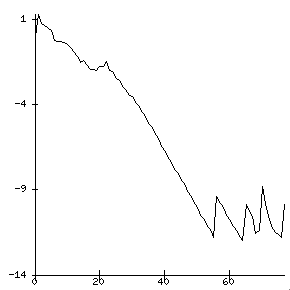
\includegraphics[width=.31\textwidth]{figures/monitor}
  \hfill
  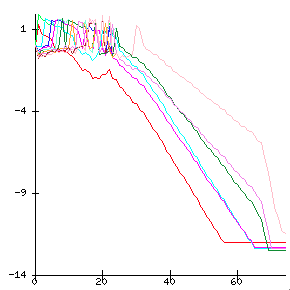
\includegraphics[width=.31\textwidth]{figures/monitorall}
  \hfill
  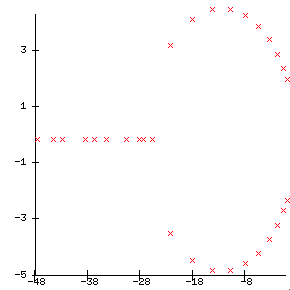
\includegraphics[width=.31\textwidth]{figures/ploteigs}
  \caption{\label{fig:plot}Graphical output in \slepc: default convergence monitor (left), simultaneous convergence monitor for all eigenvalues (middle) and eigenvalue plot (right).}
\end{figure}

	The two previously mentioned monitors have an alternative version (\Verb!*_all!) that processes all eigenvalues instead of just the first one. Figure \ref{fig:plot} (middle) corresponds to the same example but with \Verb!-eps_monitor_lg_all!. Note that these variants have a side effect: they force the computation of all error estimates even if the method would not normally do so. 

	A less verbose textual monitor is \Verb!-eps_monitor_conv!, which simply displays the iteration number at which convergence takes places.
\begin{Verbatim}[fontsize=\footnotesize,numbers=none]
   $ ./ex9 -n 200 -eps_nev 12 -eps_tol 1e-12 -eps_monitor_conv

    56 EPS converged value (error) #0 4.64001e-06+2.13951i (9.82993423e-13)
    56 EPS converged value (error) #1 4.64001e-06-2.13951i (9.82993423e-13)
    65 EPS converged value (error) #2 -0.674926+2.52867i (4.58639033e-13)
    65 EPS converged value (error) #3 -0.674926-2.52867i (4.58639033e-13)
    65 EPS converged value (error) #4 -1.79963+3.03259i (5.24172024e-13)
    65 EPS converged value (error) #5 -1.79963-3.03259i (5.24172024e-13)
    69 EPS converged value (error) #6 -3.37383+3.55626i (3.17374477e-13)
    69 EPS converged value (error) #7 -3.37383-3.55626i (3.17374477e-13)
    70 EPS converged value (error) #8 -5.39714+4.03398i (4.08586434e-13)
    70 EPS converged value (error) #9 -5.39714-4.03398i (4.08586434e-13)
    77 EPS converged value (error) #10 -7.86906+4.41229i (9.08070733e-13)
    77 EPS converged value (error) #11 -7.86906-4.41229i (9.08070733e-13)
\end{Verbatim}

Note that several monitors can be used at the same time.

Finally, the options database key \Verb!-eps_plot_eigs! instructs \slepc to plot the computed approximations of the eigenvalues at the end of the process. See Figure \ref{fig:plot} (right) for an example.

%---------------------------------------------------
\section{Advanced Usage}

	This section includes the description of advanced features of the eigensolver object. Default settings are appropriate for most applications and modification is unnecessary for normal usage.

\subsection{Initial Guesses}

	In this subsection, we consider the possibility of providing initial guesses so that the eigensolver can exploit this information to get the answer faster.

	Most of the algorithms implemented in \ident{EPS} iteratively build and improve a basis of a certain subspace, which will eventually become an eigenspace corresponding to the wanted eigenvalues. In some solvers such as those of Krylov type, this basis is constructed starting from an initial vector, $v_1$, whereas in other solvers such as those of Davidson type, an arbitrary subspace can be used to start the method. By default, \ident{EPS} initializes the starting vector or the initial subspace randomly. This default is a reasonable choice. However, it is also possible to supply an initial subspace with the command
	\findex{EPSSetInitialSpace}
	\begin{Verbatim}[fontsize=\small]
	EPSSetInitialSpace(EPS eps,PetscInt n,Vec *is);
	\end{Verbatim}
In some cases, a suitable initial space can accelerate convergence significantly, for instance when the eigenvalue calculation is one of a sequence of closely related problems, where the eigenspace of one problem is fed as the initial guess for the next problem.

Note that if the eigensolver supports only a single initial vector, but several guesses are provided, then all except the first one will be discarded. One could still build a vector that is rich in the directions of all guesses, by taking a linear combination of them, but this is less effective than using a solver that considers all guesses as a subspace.

\subsection{Dealing with Deflation Subspaces}

	In some applications, when solving an eigenvalue problem the user wishes to use a priori knowledge about the solution. This is the case when an invariant subspace has already been computed (e.g., in a previous \ident{EPSSolve} call) or when a basis of the null-space is known.

	Consider the following example. Given a graph $G$, with vertex set $V$ and edges $E$, the Laplacian matrix of $G$ is a sparse symmetric positive semidefinite matrix $L$ with elements
$$l_{ij}=\left\{\begin{array}{cl}
         d(v_i) & \mathrm{if}\;i=j\\
         -1 & \mathrm{if}\;e_{ij}\in E\\
         0&\mathrm{otherwise}
\end{array}\right.$$
where $d(v_i)$ is the degree of vertex $v_i$. This matrix is singular since all row sums are equal to zero. The constant vector is an eigenvector with zero eigenvalue, and if the graph is connected then all other eigenvalues are positive. The so-called Fiedler vector is the eigenvector associated with the smallest nonzero eigenvalue and can be used in heuristics for a number of graph manipulations such as partitioning. One possible way of computing this vector with \slepc is to instruct the eigensolver to search for the smallest eigenvalue (with \ident{EPSSetWhichEigenpairs} or by using a spectral transformation as described in next chapter) but preventing it from computing the already known eigenvalue. For this, the user must provide a basis for the invariant subspace (in this case just vector $[1,1,\ldots,1]^T$) so that the eigensolver can \emph{deflate} this subspace. This process is very similar to what eigensolvers normally do with invariant subspaces associated with eigenvalues as they converge. In other words, when a deflation space has been specified, the eigensolver works with the restriction of the problem to the orthogonal complement of this subspace.

	The following function can be used to provide the \ident{EPS} object with some basis vectors corresponding to a subspace that should be deflated during the solution process. 
	\findex{EPSSetDeflationSpace}
	\begin{Verbatim}[fontsize=\small]
	EPSSetDeflationSpace(EPS eps,PetscInt n,Vec *defl)
	\end{Verbatim}
The value \texttt{n} indicates how many vectors are passed in argument \texttt{defl}.

	The deflation space can be any subspace but typically it is most useful in the case of an invariant subspace or a null-space. In any case, \slepc internally checks to see if all (or part of) the provided subspace is a null-space of the associated linear system (see \S\ref{sec:lin}). In this case, this null-space is passed to the linear solver (see \petsc's function \texttt{KSPSetNullSpace}) to enable the solution of singular systems. In practice, this allows the computation of eigenvalues of singular pencils (i.e., when $A$ and $B$ share a common null-space).

\subsection{Orthogonalization}
\label{sec:orthog}

	Internally, eigensolvers in \ident{EPS} often need to orthogonalize a vector against a set of vectors (for instance, when building an orthonormal basis of a Krylov subspace). This operation is carried out typically by a Gram-Schmidt orthogonalization procedure. The user is able to adjust several options related to this algorithm, although the default behavior is good for most cases, and we strongly suggest not to change any of these settings. This topic is covered in detail in \hyperlink{str}{[STR-1]}.

\subsection{Computing a Large Portion of the Spectrum}
\label{sec:large-nev}

We now consider the case when the user requests a relatively large number of eigenpairs (the related case of computing all eigenvalues in a given interval is addressed in \S\ref{sec:slice}). To fix ideas, suppose that the problem size (the dimension of the matrix, denoted as \texttt{n}), is in the order of 100,000's, and the user wants \texttt{nev} to be approximately 5,000 (recall the notation of \ident{EPSSetDimensions} in \S\ref{sec:defprob}).

The first comment is that for such large values of \texttt{nev}, the rule of thumb suggested in \S\ref{sec:defprob} for selecting the value of \texttt{ncv} ($\mathtt{ncv}\geq2\cdot\mathtt{nev}$) may be inappropriate. For small values of \texttt{nev}, this rule of thumb is intended to provide the solver with a sufficiently large subspace. But for large values of \texttt{nev}, it may be enough setting \texttt{ncv} to be slightly larger than \texttt{nev}.

The second thing to take into account has to do with costs, both in terms of storage and in terms of computational effort. This issue is dependent on the particular eigensolver used, but generally speaking the user can simplify to the following points:
\begin{enumerate}
\item It is necessary to store a basis of the subspace, that is, \texttt{ncv} vectors of length \texttt{n}.
\item A considerable part of the computation is devoted to orthogonalization of the basis vectors, whose cost is roughly of order $\mathtt{ncv}^2\cdot\mathtt{n}$.
\item Within the eigensolution process, a projected eigenproblem of order \texttt{ncv} is built. At least one dense matrix of this dimension has to be stored.
\item Solving the projected eigenproblem has a computational cost of order $\mathtt{ncv}^3$. Typically, such problems need to be solved many times within the eigensolver iteration.
\end{enumerate}

It is clear that a large value of \texttt{ncv} implies a high storage requirement (points 1 and 3, especially point 1), and a high computational cost (points 2 and 4, especially point 2). However, in a scenario of such big eigenproblems, it is customary to solve the problem in parallel with many processors. In that case, it turns out that the basis vectors are stored in a distributed way and the associated operations are parallelized, so that points 1 and 2 become benign as long as sufficient processors are used. Then points 3 and 4 become really critical since in the current \slepc version the projected eigenproblem (and its associated operations) are not treated in parallel. In conclusion, the user must be aware that using a large \texttt{ncv} value introduces a serial step in the computation with high cost, that cannot be amortized by increasing the number of processors. 

From \slepc 3.0.0, another parameter \texttt{mpd} has been introduced to alleviate this problem. The name \texttt{mpd} stands for maximum projected dimension. The idea is to bound the size of the projected eigenproblem so that steps 3 and 4 work with a dimension of \texttt{mpd} at most, while steps 1 and 2 still work with a bigger dimension, up to \texttt{ncv}. Suppose we want to compute \texttt{nev}=5000. Setting \texttt{ncv}=10000 or even \texttt{ncv}=6000 would be prohibitively expensive, for the reasons explained above. But if we set e.g. \texttt{mpd}=600 then the overhead of steps 3 and 4 will be considerably diminished. Of course, this reduces the potential of approximation at each outer iteration of the algorithm, but with more iterations the same result should be obtained. The benefits will be specially noticeable in the setting of parallel computation with many processors.

Note that it is not necessary to set both \texttt{ncv} and \texttt{mpd}. For instance, one can do
\begin{Verbatim}[fontsize=\small]
	$ ./program -eps_nev 5000 -eps_mpd 600
\end{Verbatim}

\subsection{Computing Interior Eigenvalues with Harmonic Extraction}
\label{sec:harmonic}

The standard Rayleigh-Ritz projection procedure described in \S\ref{sec:eig} is most appropriate for approximating eigenvalues located at the periphery of the spectrum, especially those of largest magnitude. Most eigensolvers in \slepc are restarted, meaning that the projection is carried out repeatedly with increasingly good subspaces. An effective restarting mechanism, such as that implemented in Krylov-Schur, improves the subspace by realizing a filtering effect that tries to eliminate components in the direction of unwanted eigenvectors. In that way, it is possible to compute eigenvalues located anywhere in the spectrum, even in its interior.

Even though in theory eigensolvers could be able to approximate interior eigenvalues with a standard extraction technique, in practice convergence difficulties may arise that prevent success. The problem comes from the property that Ritz values (the approximate eigenvalues provided by the standard projection procedure) converge from the interior to the periphery of the spectrum. That is, the Ritz values that stabilize first are those in the periphery, so convergence of interior ones requires the previous convergence of all eigenvalues between them and the periphery. Furthermore, this convergence behaviour usually implies that restarting is carried out with bad approximations, so the restart is ineffective and global convergence is severely damaged.

Harmonic projection is a variation that uses a target value, $\tau$, around which the user wants to compute eigenvalues (see, e.g., \citep{Morgan:2006:HRA}). The theory establishes that harmonic Ritz values converge in such a way that eigenvalues closest to the target stabilize first, and also that no unconverged value is ever close to the target, so restarting is safe in this case. As a conclusion, eigensolvers with harmonic extraction may be effective in computing interior eigenvalues. Whether it works or not in practical cases depends on the particular distribution of the spectrum.

In order to use harmonic extraction in \slepc, it is necessary to indicate it explicitly, and provide the target value as described in \S\ref{sec:defprob} (default is $\tau=0$). The type of extraction can be set with:
	\findex{EPSSetExtraction}
	\begin{Verbatim}[fontsize=\small]
	EPSSetExtraction(EPS eps,EPSExtraction extr);
	\end{Verbatim}
Available possibilities are \texttt{EPS\_RITZ} for standard projection and \texttt{EPS\_HARMONIC} for harmonic projection (other alternatives such as refined extraction are still experimental).

A command line example would be:
	\begin{Verbatim}[fontsize=\small]
	$ ./ex5 -m 45 -eps_harmonic -eps_target 0.8 -eps_ncv 60
	\end{Verbatim}
The example computes the eigenvalue closest to $\tau=0.8$ of a real non-symmetric matrix of order 1035. Note that \texttt{ncv} has been set to a larger value than would be necessary for computing the largest magnitude eigenvalues. In general, users should expect a much slower convergence when computing interior eigenvalues compared to extreme eigenvalues. Increasing the value of \texttt{ncv} may help.

Currently, harmonic extraction is available in the default \ident{EPS} solver, that is, Krylov-Schur, and also in Arnoldi, GD, and JD.

\subsection{Balancing for Non-Hermitian Problems}
\label{sec:balancing}

In problems where the matrix has a large norm, $\|A\|_2$, the roundoff errors introduced by the eigensolver may be large. The goal of balancing is to apply a simple similarity transformation, $DAD^{-1}$, that keeps the eigenvalues unaltered but reduces the matrix norm, thus enhancing the accuracy of the computed eigenpairs. Obviously, this makes sense only in the non-Hermitian case. The matrix $D$ is chosen to be diagonal, so balancing amounts to scaling the matrix rows and columns appropriately.

In \slepc, the matrix $DAD^{-1}$ is not formed explicitly. Instead, the operators of Table \ref{tab:op} are preceded by a multiplication by $D^{-1}$ and followed by a multiplication by $D$. This allows for balancing in the case of problems with an implicit matrix.

A simple and effective Krylov balancing technique, described in \citep{Chen:2000:BSM}, is implemented in \slepc. The user calls the following subroutine to activate it.
	\findex{EPSSetBalance}
	\begin{Verbatim}[fontsize=\small]
	EPSSetBalance(EPS eps,EPSBalance bal,PetscInt its,PetscReal cutoff);
	\end{Verbatim}
Two variants are available, one-sided and two-sided, and there is also the possibility for the user to provide a pre-computed $D$ matrix.
